\chapter{화상회의 적용}

이 절에서는 화상회의에서 카멜레온을 사용하여 워터마크를 삽입하고 유출
영상으로부터 워터마크를 추출하는 과정을 설명한다. 호스트가 서버에 회의 참석자
명단을 전달하면 서버는 워터마크 메시지를 생성하여 각 PC에 전달하고, 각 PC는
전달받은 메시지를 이용하여 워터마크 화면을 생성한다. 영상이 유출되면, 기업은
워터마크를 추출하여 호스트와 출처를 확인하고, 워터마크 메시지를 서버에 전달한다.
서버는 전달받은 메시지와 호스트 키를 사용하여 진위성을 확인할 수 있다. 이 절에서
설명하는 과정은 카멜레온을 사용할 수 있는 기본적인 방법 중 하나일 뿐, 반드시 이
과정을 준수할 필요는 없다.

\section{워터마크 삽입}

카멜레온이 워터마크 메시지를 생성하기 위해서는 카멜레온 서버는 모든 회의
참석자의 식별정보와 키를 가지고 있어야 한다. 이는 사전에 회원가입 등을 통해
얻는다. 호스트는 회의를 개설하고 카멜레온 서버에 회의 참석자 명단을 전달한다.
서버는 명단을 확인하고, 각 참석자 PC에 맞는 워터마크 메시지를 전달한다. 이 때
메시지는 사전에 가지고 있던 식별정보와 키를 이용하여 생성한다. 각 PC는 메시지를
텍스트 워터마크와 QR 코드 워터마크로 생성하여 화면에 출력한다. 이로써 모든 회의
참석자는 자신에 맞는 워터마크가 삽입된 회의 화면을 볼 수 있다. 그림
\ref{fig:wm_encoding}은 위 과정을 나타낸다.
\begin{figure}[ht]
    \vspace{10pt}
    \centering
    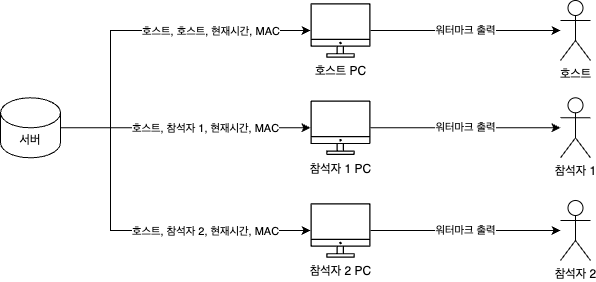
\includegraphics[width=0.7\textwidth]{imgs/wm_encoding.png}
    \caption{워터마크 삽입 과정}
    \label{fig:wm_encoding}
\end{figure}

\section{워터마크 추출}

유출영상이 심하게 훼손되었다면, 해당 영상은 가치가 없으므로 워터마크를 추출할
필요가 없다. 훼손이 적고, 텍스트 워터마크나 QR 코드 워터마크가 추출 가능할
정도로 남아 있다면, 이를 추출하여 소유자, 출처, 진위성을 확인할 수 있다.

해당 영상을 소유하고 있는 기업 또는 회의 호스트는 남아있는 워터마크를 추출 및
조합하여 워터마크 메시지를 생성한다. 메시지로부터 소유자와 출처를 확인할 수
있다. 진위성을 확인하기 위해 워터마크 메시지를 서버에 전달한다. 서버는 받은
메시지에서 호스트를 확인하고 이에 해당하는 키를 사용하여 MAC을 계산한다. 만약
계산한 값이 메시지 내 MAC과 일치한다면, 메시지 변조가 없음을 진위성 여부
요청자에게 알린다. 그림 \ref{fig:wm_decoding}는 위 과정을 그림으로 나타낸다.
\begin{figure}[ht]
    \vspace{10pt}
    \centering
    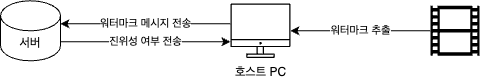
\includegraphics[width=0.7\textwidth]{imgs/wm_decoding.png}
    \caption{워터마크 추출 과정}
    \label{fig:wm_decoding}
\end{figure}